\chapter{Design and implementation}

In previous chapter we discussed how multiple assistance ways provided within Computer Aided Translation systems relate to our novel assistance tool. Further, we reviewed previous paraphrasing approaches highlighting their similarities and difference with technique we use to search paraphrases. And finally we provided a brief overview of phrase-based Statistical Machine Translation to introduce origins of the search graph, the data structure used by us as main source for paraphrasing.

Current chapter will provide detailed description of work that was carried out during the project. We will start by analysing requirements for a paraphrasing service within CAT environment. After that we will describe an iterational design and implementation process we applied to develop working version of such service. Major design decision that were made during this work will be introduced and justified. 

\section{Analysing requirements}

As mentioned earlier, an essential aspect of our paraphrasing approach is that it aims to provide a real-time targeted paraphrase search. Unlike previous efforts discussed by us before, we consider an interactive environment where queries are sent by users and executed against our data model. The results of these queries after being dynamically filtered and ranked using various heuristics are returned back to user. In this section we will list main requirements that were considered during the design stage.

\textbf{Integration with existing CAT software}. Taking into account that most of modern CAT implementations are providing web based service (Caitra, CASMACAT, MateCAT), we also employed the client-server architecture to design our paraphrasing service. As a result it might be easily attached as a module to the services provided online. Moreover, our service could be hosted as a standalone service and integrated with desktop translation software by providing an API. This way our paraphrasing assistance might be accessible from all major types of CAT applications.

\textbf{Reusing results of machine translation}. Another important feature of our paraphrasing system is being able to produce paraphrases using only data available as a result of machine translation carried out to provide other assistance types. We designed our implementation to support translation output generated by Moses \cite{koehn2007moses}. The process of retrieving and processing search graph will be reviewed by us in Section 3.2.

\textbf{Importance of ranking}. Quality of final ranking of the paraphrasing options is crucial requirement for our tool that aims to provide an interactive service. Indeed, basic concepts of Human-Computer Interaction suggest that paraphrasing options displayed to users will be efficient only in case if there are no more than seven options on the screen at a time. This means that it is important to rank top results in a way that they will contain at least one good paraphrase. Features that we exploited for ranking as well as a dynamic system of filters and sorters that we applied to improve top results will be described in Section 3.5.  

\textbf{Paraphrasing granularity}. Various levels of paraphrase granularity are studied. In case of entire sentences the task is known as \textit{sentential} (or \textit{clausal}) paraphrasing, for shorter items it is called \textit{lexical} (or \textit{phrasal}) paraphrasing. For our project we investigated only lexical paraphrases, motivating this decision by the fact that other assistance tools within a CAT system may already provide multiple translation options for entire sentence. For example, results of translation by using different bilingual parallel corpora could be provided. We also acknowledge that within scope of lexical paraphrases there is a further separation into two classes that correspond to shorter and longer phrases. Both cases were considered by us during evaluation.

We also took into account findings presented in \cite{simard2005studying}, which analyses usage patterns of another assistance tool, bilingual concordancer. Authors suggest that average length of the input query is 2-3 words. Parallels between this assistance way and ours were discussed in previous chapter. Considering these similarities we expect of average paraphrasing query length to be the same.

\textbf{Realtime experience}. Another requirement for our interactive tool is providing paraphrasing options as fast as possible. Our tool will not be useful if returning results takes longer than time user spends on manual paraphrasing. 

\textbf{Coexistence with manual editing}. While our tool aims to be used in order to fix erroneous part in the translation by getting the corrected paraphrase automatically, we acknowledge that final high quality translation cannot be achieved only by using paraphrasing. An ability to manually post-edit translation is crucial. Designing our approach we considered that it will be used in an environment where translation could be altered by user at any time.  

\section{Preparing data}

\subsection{Retrieving search graph dump file}

A representation of the search graph, described by us in Section 2.3, could be optionally returned by Moses using \textsf{-output-search-graph FILE} parameter. The resulting text file contains list of hypotheses that were considered during the decoding stage. Each line in the file represents such hypothesis. Content of file is ordered by sentence identifiers that appear in the beginning of each line. This identifiers indicate to the sentence that was being translated when the hypothesis formed. The hypotheses are in one of three possible formats.

The \textit{initial hypothesis} refers to the empty hypothesis that is used as starting point in process of hypothesis expansion. This hypotheses have a simple structure and don't carry any additional information:

\begin{verbatim}
0 hyp=0 stack=0
\end{verbatim}

The \textit{regular hypothesis} encodes information about translation decisions that were made by the decoder in a given state. Sample regular hypothesis has the following format:

\begin{verbatim}
0 hyp=10 stack=1 back=0 score=-1.497 transition=-1.497 forward=3437
fscore=-8.900 covered=0-0 out=del Parlamento
\end{verbatim}

The line starts with sentence identifier which is followed by a unique hypothesis identifier \textsf{hyp=10}. This identifier is used to reference hypotheses. The stack in which hypothesis is placed during stack decoding is identified by \textsf{stack=1}, this is also the number of words covered in original input.

The next attribute \textsf{back=0} is a reference to the previous hypothesis, in this case it refers to the initial empty hypothesis. This means that current hypothesis represents the first addition of a translation option. Overall score of current partial translation is expressed as \textsf{score=-1.497}, which derives from a log-probability, calculated given machine translation models. The cost of transition to current state is available as \textsf{transition=-1.497}. 

After finalising the translation, hypothesis attributes are enriched by adding information about the best forward step to the end of the graph \textsf{forward=3437} and the best score after this step \textsf{fscore=-8.900}. Original sentence coverage information is available in following format \textsf{covered=0-0}, where \textsf{0-0} indicates covered interval. Finally, the last attribute \textsf{out=del Parlamento} contains the translation option that was added by introducing current hypothesis.

The third type of hypotheses are \textit{recombined hypotheses}. These hypotheses are omitted as a result of recombination process that was reviewed by us in Section 2.3.5. Recombined hypotheses have following format

\begin{verbatim}
0 hyp=734 stack=2 back=24 score=-2.684 transition=-1.226 
recombined=731 forward=8037 fscore=-7.962 covered=3-3 out=de Apoyo
\end{verbatim}

Here additional attribute \textsf{recombined=731} indicates to the hypothesis with a better score, with which current hypothesis was recombined.

Another option to fetch the information generated during decoding is executing Moses with \textsf{-verbose 3} parameter. This way detailed logs will be provided by the system. The resulting output will contain mostly discarded hypotheses and will not have information about the best path that is being added in case of the method we described earlier. That is why we prefer using the \textsf{-output-search-graph} option instead.

More details are available at [http://goo.gl/6RYbDK]

\subsection{Preprocessing data for paraphrasing}

For initial testing purposes we used Moses to translate set of 3000 Russian sentences from news domain (\textit{newstest2012b}) into English. The resulting search graph dump file was about 5.7GB. In order to process it efficiently we decided to encode information from this file into a relational database. We developed a small Python script that parsed each line in the search graph file and mapped the attributes into a dictionary. The dictionary was then stored in an SQLite database. The resulting transformation reduced size of our graph representation to 2.3GB. Moreover, main benefit of having our graph stored in a relational database was being able to run SQL queries against it. 

\section{Project design outline}

In this section we want to introduce high-level structure of the project listing it's main components and their short descriptions. Following sections will provide more details about implementation of these components. As it was mentioned before, our service designed using client-server architecture. Client-side implementation may vary depending on particular CAT software within which paraphrasing service is provided.
That is why integrating our solution with a particular CAT system was out of the scope of current work. However we implemented a simple web based interfaces to test usability and feasibility of our tool. 

Our server-side implementation is also designed as a proof of the concept and currently supports only paraphrasing of sentences that are available in the preprocessed search graph database. The production of this database graph was reviewed in previous section. In practice it could be executed as an initialisation step triggered after the machine translation for post-editing is produced. Simple sequence of components that are used to process paraphrasing requests are illustrated in Figure 3.1.

\begin{figure}
 \centering 
 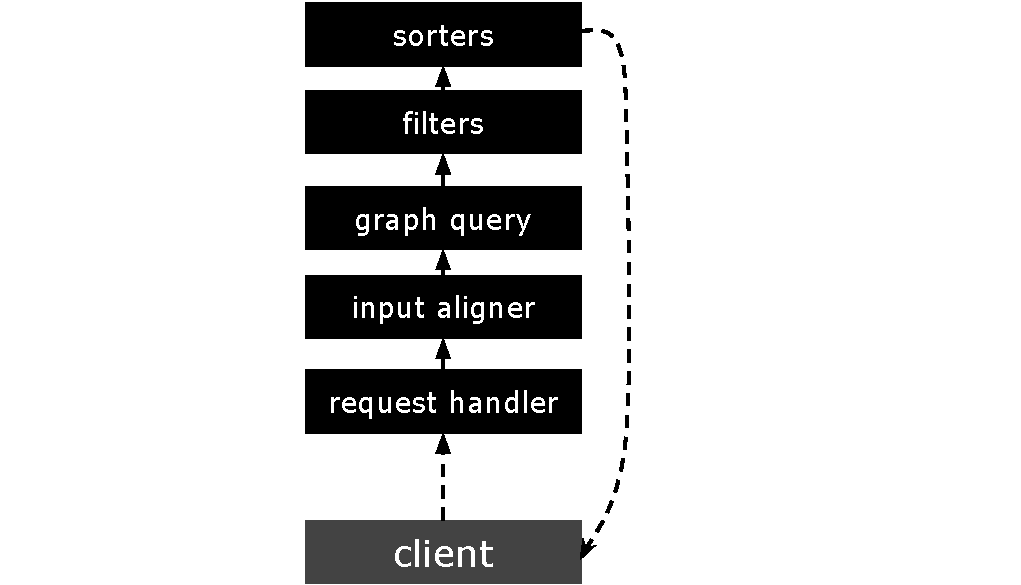
\includegraphics{g/system-outline.pdf}
 \caption{Paraphrasing request handling}
\end{figure}

\subsection{Sending requests from client}

Simple integration of paraphrasing service into a Computer Aided Translation interface will require adding a button labeled ``Paraphrase Selection'' near the active translation edition box. The button will be enabled only in case if user selects part of translation text using mouse cursor. Once clicked, button will fire an event that will send a paraphrasing request. The requests from clients are sent over HTTP protocol using AJAX technology. Figure 3.2 illustrates English to Russian translation setup in the CASMACAT system, where user selects part of translation provided for post-editing and paraphrase button is activated.

\begin{figure}
 \centering
 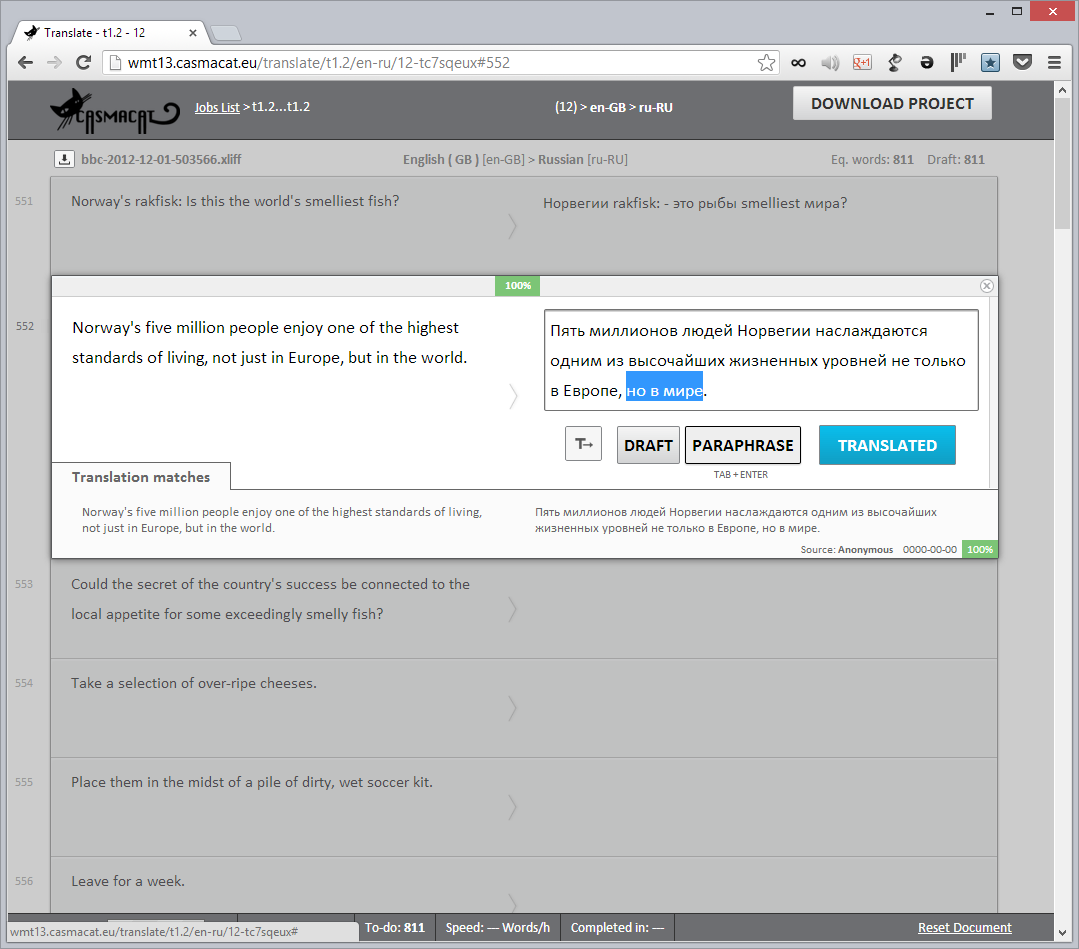
\includegraphics[scale=0.5]{g/screenshot.png}
 \caption{Sample screenshot of paraphrasing client UI}
\end{figure}

\subsection{Request handler}

The role of request handler is simply to intercept messages from client-side and to transform them into native easy to use data structures. In our implementation we used Werkzeug WSGI toolkit which is freely available for Python.

\subsection{Input aligner}

Before user's paraphrasing query is executed against our graph database, it is being aligned with corresponding part of the original source language sentence. The main reasoning behind this step is making sure that our paraphrasing will not produce duplicated translation by capturing partial translation of a phrase that was not originally requested by user. In this process we are interested only in retrieving pointers to original sentence parts that correspond to user selection, fetching original language phrases is not required.

\subsection{Graph query execution}

Having required information about coverage, system executes a query against the search graph database. This is achieved by transforming search constraints into an SQL query. Depending on phrase length and other phrase specific features several sequential SQL queries could be executed. The results represent a list of unfiltered translation options that have high probability of being suitable paraphrases to user selection. Each translation option is paired with data about corresponding hypothesis scores, that are used in further stages of paraphrasing workflow.

\subsection{Filters, score functions and sorters}

The results retrieved from database usually are very redundant and have formatting issues. Thus the next step is filtering them. After that using sorter functions are used to generate final ranking. These steps encapsulate the most significant parts of the paraphrasing algorithm. In order to experiment with various filtering and ranking techniques we have implemented a dynamic system of attachable filters and sorters. This way we were able to easily produce multiple variations of our approach and evaluate all of them against one test suite. Importantly, another benefit of this dynamic modular system is that depending on user query we can execute different sets of filters and sorters. For example, some filters could be efficiently used only for short phrases, while others are suitable for long inputs. 

\section{Implementation details}

In this section implementation details of the design components will be provided. We will start by consistently discussing the parts that are directly involved in paraphrasing. Description of each component will also contain problematic cases and their solutions discovered by us. 

\subsection{Implementing input aligner}

Input aligner detects coverage of user selection submitted for paraphrasing. Later paraphraser uses this coverage information to ensure that results do not contain words with meanings that are not part of the original selection. Information about coverage is available within machine translation output. The translation output for each sentence is formatted as in the following sample:

\begin{verbatim}
Indiana |0-0| became the |1-1| first state |2-3| 
to impose |4-4| such a requirement . |5-7|
\end{verbatim}

Here each phrase in translation is followed by coverage details. These details are surrounded by vertical bars and contain start and end positions separated by a hyphen. For example, from this part: \texttt{first state |2-3|}, we can see that ``first state'' phrase corresponds to words in the original sentence with indices 2 and 3. We are only interested in these indices as the corresponding words do not carry useful information for paraphrasing.

The alignment is achieved by matching the user's paraphrasing input with the machine translation output sentence. For now, we consider that user's selection matches part of unmodified translation output. Later we will describe cases when user requests paraphrasing after manually editing the translation. The alignment procedure includes following steps:

\begin{enumerate}
  \item \textbf{Parsing output sentence}. We start by extracting coverage information from the output sentence and storing it in a separate data structure. The coverage data structure represents mapping between translation output and original sentence expressed in word indicies. It is also possible to execute this transformation during data preprocessing described in previous section. 
  \item \textbf{Locating input}. On this step we match user's paraphrasing input with the translation. We express input words using indicies of corresponding words in translation.
  \item \textbf{Finding involved intervals}. The final step is merging results of previous two steps to find indicies of words in original sentence that correspond to user's selection. 
\end{enumerate}

For example, application of step 1 to our sample sentence will produce the following coverage mapping:

\begin{verbatim}
|0-0| : |0-0|, |1-2| : |1-1|, |3-4| : |2-3|, 
|5-6| : |4-4|, |7-10| : |5-7|
\end{verbatim}

On step 2, given \texttt{became the first state} as user's input, we will get:

\begin{verbatim}
became [1], the [2], first[3], state[4]
\end{verbatim}

Considering that user can submit only one selection at a time this mapping will always be sequential.
Finding corresponding interval for each index in the input representation, we get following coverage information:

\begin{verbatim}
became the first state |1-3| (1-1, 2-3) 
\end{verbatim}

Having this information we can consider the alignment to be complete. The described process is straightforward in case of our example. However there are situations when additional heuristics are required for paraphrasing alignment.

One minor problem during alignment is dealing with \emph{selections that contain only some parts of words}. An example of such selection could be \texttt{rst state}. This situations are prevented on client-side by appending the rest of the word in case if most of it is selected and omitting the partial otherwise.

Another problem is with \emph{selections that contain only some parts of phrases}. Coverage information available for translation is provided on phrase level and do not contain word by word mapping. For user's input \texttt{became the first}, our aligner will produce the same coverage information as for \texttt{became the first state}. However, the word with index 3 in original sentence means ``state'' and it is not covered by \texttt{became the first}. During current project this problem was solved by automatically extending user input to match the whole phrases. We also considered one exceptional case, when the partial phrase contains only function words. Given \texttt{the first state} as paraphrasing input, instead of extending it into \texttt{became the first state}, we reduce it by removing \texttt{the}. Alternatively, this problem could be tackled by using additional detailed word alignment information.

Finally, alignment logic gets more complicated in case when user submits selection after manually editing translation. In this case user input may not exactly match any part of translation output. If user changes are minor, for example fixing agreement between words, our alignment approach can still be used by introducing \emph{fuzzy matching}. These matching is based on edit distance. While this practice is dangerous in case of short selections, with multi-word inputs we can take into account the fact that words should match parts of the translation output sequentially. For example, given \texttt{told us that war} as input, matching the word \texttt{us} should be correct for the following sentence: 

\begin{verbatim}
the us president told us the war on terror must come to an end
\end{verbatim}

The logic of such fuzzy alignment can be expressed in terms of Hidden Markov Models (HMM). As these models were not used in the core paraphrasing implementation, we will not provide detailed definition of them. In short, HMMs are used to model systems that represent a process with hidden states, while for these states it is true that future and past states are conditionally independent given a number of present states.

For the alignment case, each word in the translation output represents an observation. We denote observations as $w_{i}$. Each observation corresponds to one of the hidden states that are words in user input, plus special state ``none'', which means that observation does not correspond to any input word. The states are denoted as $s_{j}$. 

\begin{center}
The states sequence $s_{1}^{n}$ with highest probability given observations sequence $w_{1}^{n}$ can be expressed using the Bayes' rule in this way 
\end{center}
\begin{large}
\begin{equation}
\arg \max_{s_{1}^{n}} P(s_{1}^{n}|w_{1}^{n}) = \arg \max_{s_{1}^{n}} \frac{P(w_{1}^{n}|s_{1}^{n})P(s_{1}^{n})}{P(w_{1}^{n})}
\end{equation}
\end{large}

\begin{center}
Considering a first order HMM, we have following Markov assumption:
\end{center}
\begin{large}
\begin{equation}
P(s_{i}|s_{1}^{i-1}) = P(s_{i}|s_{i-1})
\end{equation}
\end{large}

\begin{center}
Having this assumption we can represent prior probability $P(s_{i}^{n})$ as
\end{center}
\begin{large}
\begin{equation}
P(s_{i}^{n}) = \prod^{n}_{i=1} P(s_{i}|s_{i-1})
\end{equation}
\end{large}

\begin{center}
Finally considering the following independence $P(w_{1}^{n}|s_{1}^{n}) = \prod_{i=1}^{n}P(w_{i}|s_{i})$; the fact that $P(w_{1}^{n})$ is invariant and prior probability representation from previous equation, we get this expression:
\end{center}
\begin{large}
\begin{equation}
\arg \max_{s_{1}^{n}} P(s_{1}^{n}|w_{1}^{n}) \approx  \arg \max_{s_{1}^{n}} \prod^{n}_{i=1} P(w_{i}|s_{i}) P(s_{i}|s_{i-1})
\end{equation}
\end{large}
\begin{center}
Probability $P(w_{i}|s_{i})$ from the last equation is known as \emph{sensor model} and probability $P(s_{i}|s_{i-1})$ is known as \emph{transition model}.
\end{center}

In our alignment case the sensor model is calculated using string edit distance between an observation and the states. The transition model calculation is based on the sequence of words in user input. For our example, probability of the first $w_{2}$ and second $w_{5}$ occurrences of \texttt{us} are calculated as: 

\begin{large}
\begin{equation}
P(us|w_{2}) = P(w_{2}|us) P(us|none)
\end{equation}
\end{large}
\begin{center}
Here we use $P(us|none)$, because we assume that the first word ``the'' was not matched with any of the input words and thus it is tagged as ``none''.
\end{center}

\begin{large}
\begin{equation}
P(us|w_{5}) = P(w_{5}|us) P(us|told)
\end{equation}
\end{large}
\begin{center}
Here we use $P(us|told)$, because we assume that the fourth word ``told'' was tagged to be in state \emph{told}.
\end{center}

Here $P(w_{i}|us)$ expresses probability of that $w_{i}$ corresponds to \texttt{us} from selection. And $P(us|s_{j})$ is probability that current word corresponds to \texttt{us}, given that previous word corresponds to $s_{j}$. Considering the input sequence \texttt{told us that war}, the second probability is higher.

In cases when user edits are significant, the described approach will tag all words in translation output as ``none''. In these situations, one option is to use a word aligner like GIZA++ to re-align user's current translation with original sentence and use updated coverage information. Another option is to ignore coverage and to switch to a monolingual paraphrasing, this type of paraphrasing is not supported by our approach. Our paraphrasing approach requires the user input to be a partial translation of original sentence. This requirement lets us to use search graph as data source for paraphrasing. Unfortunately, this constraint also does not let our paraphrasing approach to be used outside translation task.

Source code of both regular and fuzzy alignment implementations are available in project file named \textsf{aligner.py}. 

\subsection{Retrieving partial paraphrases from search graph}

We use the coverage information collected during alignment to construct and execute queries against search graph database. We formed this SQLite database during preprocessing step. The database contains only one table which has following fields: \texttt{sentenceId, hyp, stack, back, score, transition, recombined, forward, fscore, covered, out}. These fields correspond to the attributes available from the search graph dump file, that we described in Section 3.2. 

Queries encode a number of constraints that are required to find hypotheses that are potential partial paraphrases for user input. These constraints are:

\begin{itemize}
  \item \emph{Hypotheses should be from the same sentence}. This basic limitation significantly reduces the search space by focusing only on the search graph representation of the sentence that user currently translates.
  \item \emph{Hypotheses should be within the same coverage as user's input}. As discussed before, it is crucial to preserve same coverage after translation. This rule is related to the paraphrasing approach using bilingual parallel corpora \cite{Callison-Burch2007}. Similarly, we consider different phrases that have same translation to be paraphrases. In our case, instead of using parallel corpus, we use information generated for only one sentence. This information encoded in search graph was generated using machine translation models, that were built using parallel corpus. This fact relates our approach to the approach described by \cite{Callison-Burch2007}.
  \item \emph{Hypotheses should be ordered by score in descending order}. This requirement ensures that hypotheses that have better partial score will appear on top of the list. While having this ordering is useful for filtering and ranking, the score value depends on translation order and that is why it cannot be considered as a sole feature for final ranking decision.
\end{itemize}

While expressing the first and the last constraints in SQL is trivial, requesting hypotheses within the same coverage requires further analysis.  

In order to find all hypotheses that could be used to form final paraphrasing options we have to build queries for each possible separation of original coverage. However the number of possible ways to split coverage into phrases exponentially grows with number of words covered. For $n$ sequential words in original sentence, there are $2^{n-1}$ possible ways to group them into phrases. This could be demonstrated by defining \textsf{split (0)} and \textsf{join (1)} decisions between words, then grouping of original words could be expressed as binary sequence with length $n-1$, where $n$ is number of words. Moreover, the original coverage is not always sequential, therefore we should consider each sequential interval separately.

Considering this exponential growth, starting from cases with $n > 4$ it is not feasible to build SQL queries that reflect each possible grouping. One way to solve this problem is using grouping that was used for producing translation output. We can also use information about the best next step (\texttt{forward} and \texttt{fscore}) to detect the most useful grouping options. Here are descriptions of the operations that are carried out to retrieve hypotheses that are later used for paraphrasing following input: \texttt{first state |2-3| to impose |4-4| such a requirement. |5-7|}.

\begin{itemize}
    \item We start by finding \emph{partial paraphrases} for the first phrase in user selection. In our case this phrase is \texttt{first state}. Using SQL we query all hypotheses within current sentence that have coverage \texttt{|2-3|}. 
    \item Next, for each result we follow reference to the next best hypothesis and record it's coverage. Our goal is to collect all possible coverage types that are available for the best next steps. This way we reuse grouping that was statistically built during machine translation. For our example, two new coverage types are: \texttt{|4-4|} and \texttt{|4-5|}.
    \item After removing coverage types that are not withing overall coverage of user selection, which in our case is \texttt{|2-7|}. We run the procedure described in the previous step recursively for each new coverage type. The results of all queries are recorded in a dictionary data structure, where key represents coverage type and value contains pointers to the rows retrieved from database. For our example in the end we get three new coverage types: \texttt{|5-5|}, \texttt{|5-7|} and \texttt{|6-7|}. 
\end{itemize}

This process is also illustrated on Figure 3.3. While growth of options number in this case is significantly slower than considering all possible groupings, for longer inputs number of queries executed is still too high. Therefore for long selections our approach uses only grouping produced by decoder for translation output. Another option could be splitting longer inputs into small equal parts and then considering each part as a separate paraphrasing input. But this method produces too many partial paraphrasing options and it is not possible to assess all potential ways to join them in context of a real-time interactive system. 
 
\begin{figure}
 \centering 
 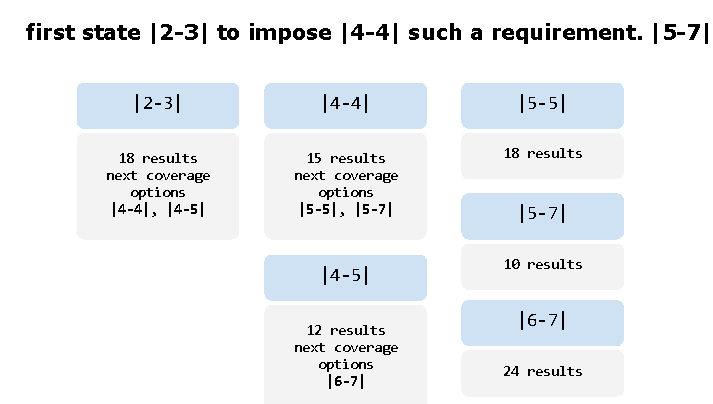
\includegraphics{g/coverage-expansion.pdf}
 \caption{Retrieving partial paraphrases with different coverage}
\end{figure}

\subsection{Merging partial paraphrases}

After running queries we get partial paraphrases stored in a dictionary, where keys represent coverage. The next step is merging this partials in paraphrasing options. We achieve this goal by using a data structure known as finite state machine (FSM). This data structure is defined by set of states, including start/end states and by list of transitions between these states. Our approach is similar to the usage of FSM for finding N-best candidate translations in a search graph which is described in \cite{Koehn2009a} Section 9.1.2. In our case we are dealing with significantly smaller part of the search graph which represents the part of the sentence that matches user input, instead of the whole sentence. Also we already have the scores calculated during translation. The key difference of our approach is that we know that the part of the translation submitted by user for paraphrasing is probably not good enough and we try to reassess scores based on this information and find alternative promising paths in the graph using various features of the hypotheses. 

We define one start state which refers to an empty string. Other states represent partial paraphrases (hypotheses) retrieved from search graph. Transitions between states mean adding partial paraphrase to form the final paraphrase. Transitions are only possible in a way that they maintain original coverage. For example, transition from state with coverage \texttt{|4-4|} is only possible to states with coverage \texttt{|5-5|} and \texttt{|5-7|}. Additional score is associated with each translation. For each state the score of outgoing transitions are high if they are expected to lead to a good paraphrase, otherwise the score is low. These scores are calculated using various features like string distance, diversity factor and language model score. For each feature there is a \emph{score function} that assesses it for a given transition and adds the result to the final score. The score functions are dynamically attachable, therefore we can easily create many versions of paraphraser that use different combinations of features for assessing transitions. 

Before constructing finite state machine, we need to clean up partial results, that contain many redundant results. We use dynamically attachable \emph{partial filters} to filter states considering similarity, function words and punctuation. The next step is adding transitions from start state to states with coverage that matches the beginning of the original overall coverage. We continue by adding transitions considering the overall coverage. The end states of our FSM are the states with coverage that matches the end of the overall coverage. A part of a sample finite state machine for our example input \texttt{first state |2-3| to impose |4-4| such a requirement. |5-7|} is illustrated on Figure 3.4.

\begin{figure}
 \centering 
 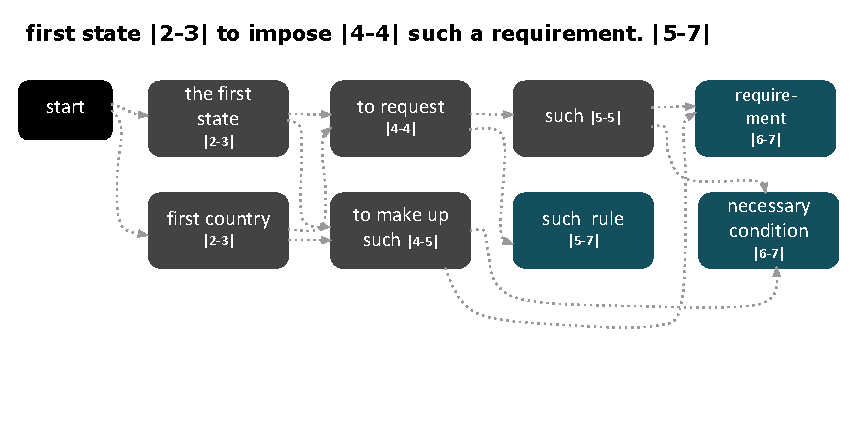
\includegraphics{g/fsm.pdf}
 \caption{A part of a sample finite state machine}
\end{figure}

After constructing a FSM, the next step is to generate the most promising paraphrasing options. In order to do so, we search for \emph{$K$ best paths} that start in the start state and end in one of the end states. A number of algorithms exist to solve this problem. One of them is \emph{Yen's algorithm} \citep{yen1971finding}. We used it's open source Python implementation called \emph{YanKSP}. For each end state we find $n$ best paths, and if we define number of end states as $t$, as result we get $K = nt$ paraphrasing options. The number of end states $t$ is significantly larger for longer phrases, we compensate it by reducing $n$. As a result the number of final results $K$ is not too large to be analysed within a real-time system.

Finally, having $K$ paraphrasing candidates our goal is to filter and sort them in order to achieve the best possible final ranking. Final ranking is crucial because only limited number of top results are displayed to user. The number of results should be small enough to keep paraphrasing decision simple for the user. On this stage filtering and sorting functionality is implemented similarly to partial filters and score functions. Again we have an optionally attachable \emph{filters} and \emph{sorters} that form final list of paraphrasing options. The filters and the sorters, in contrast with the partial filters and the score functions are applied to whole paraphrase candidates, rather than to partial paraphrases, thus they can use more assessment types. At the same time using score functions within a finite state machine has benefits, for example it helps us to preserve calculations carried out to decide whether it worth to merge two partial paraphrases or not. 

Figure 3.5 illustrates the workflow described in this section. We will continue by discussing existing filters, score functions, partial filters and sorters in the next section.

\begin{figure}
 \centering 
 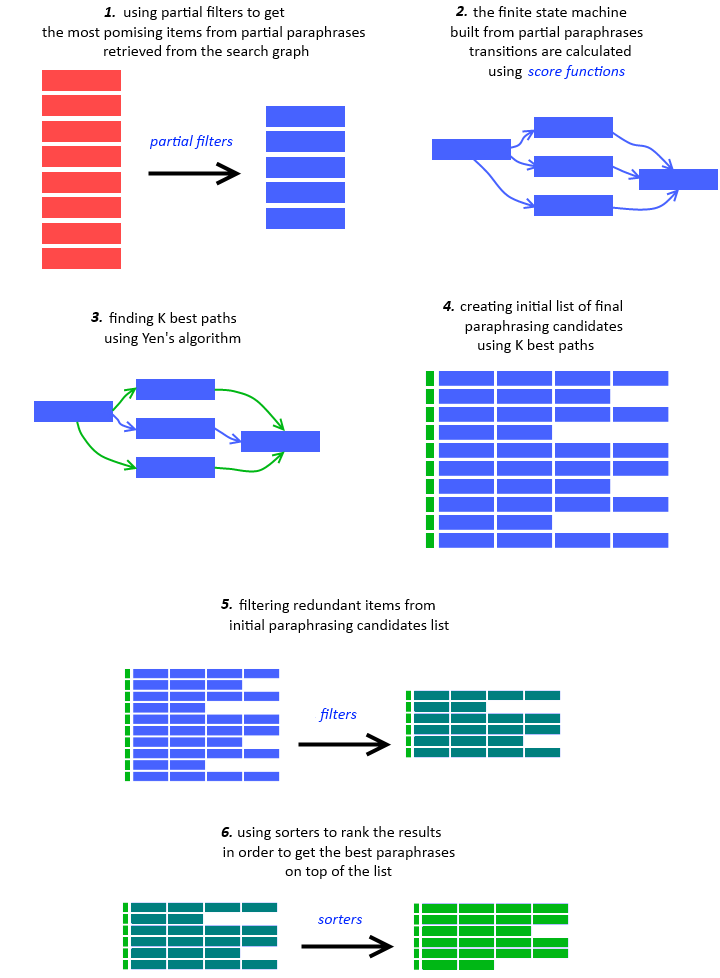
\includegraphics[scale=0.82]{g/main-workflow.png}
 \caption{This figure illustrates the main workflow of our paraphrasing approach}
\end{figure}

\subsection{Implementing functions}

One of the requirements for this project was carrying out a number of experiments to find the set of features within a search graph that are the most useful ones for achieving feasible paraphrasing results. In order to organise these experiments we designed our paraphraser in a way that some parts of it's logic are represented by dynamically attachable functions. These functions are grouped by their use cases. Each function within such a group accepts same arguments and returns result in the same format. These groups include: \emph{filters}, \emph{partial filters}, \emph{score functions} and \emph{sorters}. To implement dynamically attachable functionality we used a variation of a classic software design pattern known as \emph{Decorator} \citep{vlissides1995design}.

Here we provide a list of the implemented functions. We assign a four letter code for each function. Later these codes will be used to describe functions that were used in different experiments.

\subsubsection{Partial filters}

In previous sections we described how paraphrasing options are built using a finite state machine. States of this machine are hypotheses retrieved from search graph database. Before converting each hypotheses from database query results, we use partial filters to remove the ones that are not likely to be part of a good paraphrasing option. There are two ways to instantiate a partial filter. The first way is to construct it using a list of hypotheses in a format as we get it from database. Items of this list contain all features that are initially available in search graph attributes. After processing this list, partial filter will output a list in the same format with reduced number of items. The second way to instantiate a partial filter is to construct it using another partial filter. In this case before applying filtering logic, our partial filter will execute another partial filter and then will use it's results as initial data for filtering. Using both constructors makes it possible to build complex filters. This design solution is the variation of the Decorator pattern, we mentioned before. Following pseudocode illustrates the base class that is extended by all partial filters: 

\begin{verbatim}
abstract class PartialFilter:
    PartialFilter(Hypothesis[] hypotheses)
    PartialFilter(PartialFilter anotherFilter)
    def Hypothesis[] filter()
\end{verbatim}


Most of our partial filters aim to reduce original list of hypotheses by removing redundant items. Here we listed partial filters that were implemented during the project:

\begin{flushleft}

\textbf{\texttt{PTPF}: \textbf{Punctuation Partial Filter}} \\
We iterate the input list and remove all punctuation and special signs for each item, also we replace multiple spaces between words with one. We remove duplicates from the resulting list and return the final list.\\
\bigskip 
\bigskip 

\textbf{\texttt{SDPF}: \textbf{String Distance Partial Filter}} \\
For each item in the list we calculate Levenshtein string distance between it and the following items. If the distance is below a given threshold $t$ and it has the same coverage as current item, we remove it from the list. It's important to consider that the scores in the list are already in descending order, so we leave only the best candidates in terms of score. Having same coverage makes these score comparable. For all our experiments we used $t = 3$, because intuitively assumed that filtering items with longer distance we might lose good partial paraphrasing candidates. \\
\bigskip 

\textbf{\texttt{FWPF}: \textbf{Function Word Partial Filter}} \\
For each item we remove following items if the only difference between two strings is in function words. This way in the resulting list there are still function words. In this filter we use list of functions words available within NLTK library []. \\
\bigskip 

\end{flushleft} 

\subsubsection{Score functions}

We use score function in order to assess a transition between two steps in paraphrasing finite state machine. Similarly to partial filters score functions follow the Decorator pattern. A basic constructor for a score function requires two hypotheses that refer to source and target states. Score function outputs a normalised value between 0 and 1. 

Another constructor instantiates a score function, using other score function. In this case, source and target states are extracted from previous function. Also initial score is set to be equal to the score produced by the previous score function. After calculating score with current function, result is set to be equal to the average of two scores. A pseudocode for base score function class is listed here:

\begin{verbatim}
abstract class ScoreFunction:
    ScoreFunction(Hypothesis source, Hypothesis target)
    ScoreFunction(ScoreFunction anotherScoreFunction)
    def float calculate()
\end{verbatim}


\begin{flushleft}

\textbf{\texttt{BFSF}: \textbf{Best Forward Score Function}} \\
This function is based on similarity with the best next translation option from the search graph. It checks if target hypothesis has the same id as \texttt{forward} reference for the source hypothesis. In this case it outputs 1. Otherwise it retrieves the best next hypothesis and calculates a string distance between it and target. If distance is more than $9$, function outputs $0$. Otherwise it the result is calculated as $1-d/10$, where $d$ is the distance. Current score function uses only the reference to the best next hypothesis (\texttt{forward}) and ignores the value of the \texttt{fscore} attribute.  \\
\bigskip

\textbf{\texttt{SDSF}: \textbf{Score Difference Score Function}} \\
This function deals with the ratio between \texttt{transition} scores available from the search graph for source and target states. Output is a number between 0 and 1, calculated as:
\begin{large}
\begin{equation}
\min(\frac{score_{t}}{2 score_{s}}, 1)
\end{equation}
\end{large}
\begin{center}
Here $score_{t}$ is the target score and $score_{s}$ is the source score. \\
This expression encodes an increment in transition score between two states
\end{center}

As a result the output will be higher if transition score for target state in the search graph is higher than the transition score for source state, otherwise it will be lower. The main intuition behind this score function is that if transition score encodes the positive effect of adding particular partial translation during decoding, then following the path along which this score increases should lead to an output that has a good agreement between partial paraphrases.
\bigskip


\textbf{\texttt{LMSF}: \textbf{Language Model Score Function}} \\
This function uses language model that was used for machine translation to score the result of merging outputs of two hypotheses. In order to get language model score we use \emph{KenLM} tool in the following way:

\begin{verbatim}
echo 'this is a test' | ./moses/bin/query ~/lm/bin.lm
\end{verbatim}

This command returns a detailed score distribution. However we use use only overall total score.
\bigskip

\end{flushleft}


\subsubsection{Filters}

In contrast with partial filters, regular filters are applied to the final list of paraphrasing options. This list is generated using FSM and we still may want to remove paraphrasing candidates that are similar. Interface of this function is very similar to the interface of partial filters. Base class extended by all filters looks like:

\begin{verbatim}
abstract class Filter:
    Filter(Paraphrase[] options)
    Filter(Filter anotherFilter)
    def Paraphrase[] filter()
\end{verbatim}

Two filters implemented by us are repeating logic of the String Distance, Punctuation and the Function Word partial filters. They are correspondingly named \textbf{Punctuation String Distance Filter} (\textbf{\texttt{PTRF}}) and \textbf{Function Word Filter} (\texttt{\textbf{FNRF}}). The only novel filter is a score based filter and it's description is provided here:


\begin{flushleft}

\textbf{\texttt{SBRF}: \textbf{Score Based Filter}} \\
This simple filter removes items that have a final FSM score which is below a predefined threshold. 
The filter is used only in cases when number of results it too large to be handled by sorters. Threshold depends on number of items in the list.
\bigskip

\end{flushleft}

\subsubsection{Sorters}

Sorters are applied to the filtered list of paraphrasing candidates. These functions aim to produce best possible final ranking for the paraphrases. They have similar interface with filters, the difference is that instead of removing items, sorters reorder them in the resulting list. Sorters also have parallels with score functions as both function types try to assess quality of paraphrases. While score functions are used to test feasibility of merging two partial paraphrases, sorters are used to assess final whole paraphrasing candidates. Initial list passed to sorters is already ordered by the FSM scores. The parent class for all sorters is listed below:

\begin{verbatim}
abstract class Sorter:
    Sorter(Paraphrase[] options)
    Sorter(Sorter anotherSorter)
    def Paraphrase[] sort()
\end{verbatim}


\begin{flushleft}

\textbf{\texttt{LMBS}: \textbf{Language Model Based Sorter}} \\
In contrast with Language Model Score Function which assesses only partial phrases, Language Model Based Sorter uses the language model score for a whole sentence by replacing user input with a paraphrasing candidate. This way paraphrase is assessed in context of the surrounding words. Items in the list are rearranged by score in descending order. 
\bigskip

\textbf{\texttt{CDBS}: \textbf{Cluster Diversity Based Sorter}} \\
This sorter is based on a heuristic which assumes that more diverse results are more useful for users. Indeed, a user searching for paraphrases is likely to be looking for a way to express idea in a different way, rather that trying to fix a minor spelling mistake. To achieve more contrasting results we use simple clustering approach. We group items into clusters based on word distance. The distance is calculated similarly to the string distance, considering words as atomic units instead of characters. For clustering we use an implementation of K-Means for Python available within SciPy library []. The number of clusters $K$ is set to be equal to the number of top paraphrases displayed to user. The order within each cluster is the same as in the original list. The next step after clustering is to create output list. To do so we iteratively populate an empty list, by adding the top items from each cluster. The order of clusters depends on order of their first item in the original list. This way we achieve an output where top results are significantly different from each other, but at the same time have high scores.
\bigskip

\end{flushleft}


